\subsection{Menu}
\par Le menu est une �tape indispensable dans la cr�ation d'un jeu vid�o. Nous avons d�cid� de baser le notre sur un syst�me de pile: Chaque sc�ne s'empile les unes par dessus les autres, ainsi au plus bas de la pile vous aurez toujours le menu du d�part, puis s'empile par dessus le choix du mode de jeu, le choix du niveau, pour finir sur la sc�ne de jeu.
\par La pause s'empile encore par dessus la sc�ne de jeu, puis tout est d�pil� quand besoin pour revenir au menu principal. Le menu �tait pr�sent tr�s rapidement dans le jeu, car nous souhaitions le terminer avant de trop avancer dans le d�veloppement du jeu en lui m�me, c'est pourquoi ce dernier n'a pas chang� d'aspect graphique depuis la soutenance 2.
\par Un screenshot du menu:
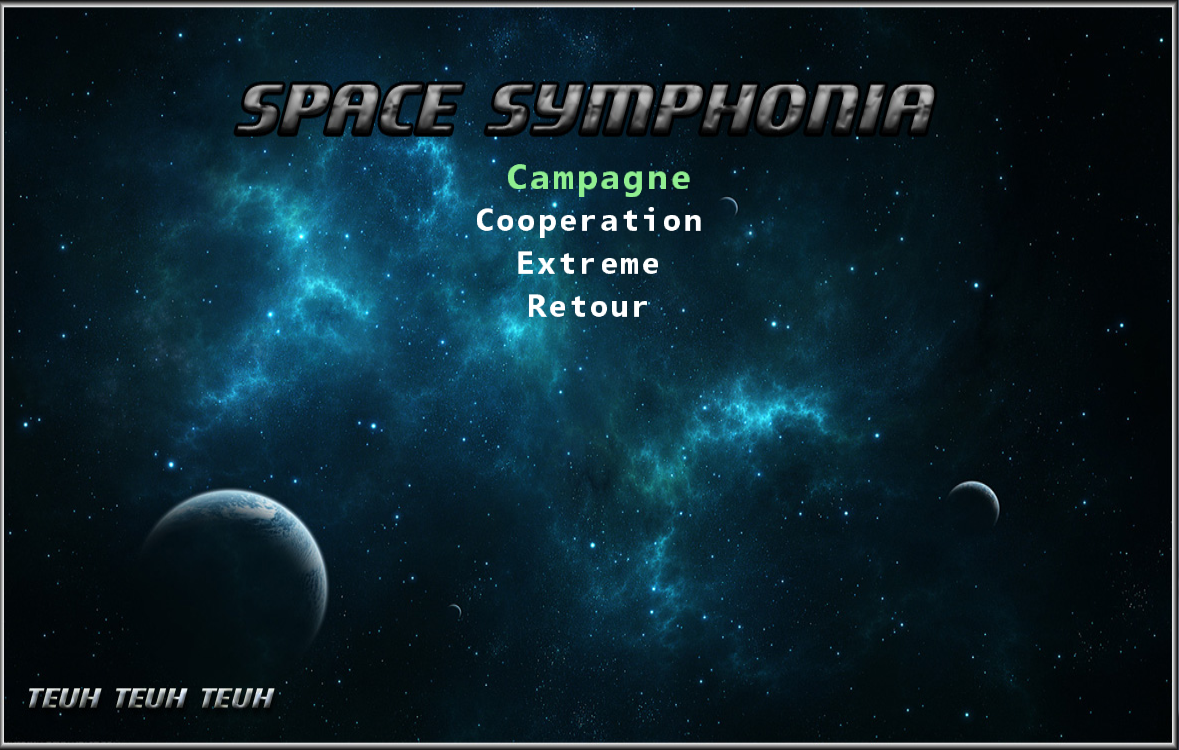
\includegraphics{images/menu1.png}
\par Le menu permet donc au joueur d'acc�der directement au jeu, mais aussi d'ouvrir l'�diteur de niveau afin de cr�er ses propres niveaux, de changer la difficult�e du jeu, de voir ses scores.
\subsubsection{Scores}
\par Dans un Shoot them all, le score est surement ce qu'il y a de plus important. Nous devions d�velopper un syst�me infaillible et performant, dans lequel le joueur pourrait se comparer � ses amis.
\par Ainsi, � chaque fin de niveaux, en mode campagne ou extr�me, le joueur est invit� � rentrer son nom. Son score est enregistr�, et est visible dans le menu partie "Scores". 
\par Dans ce menu, tous les meilleures scores par niveaux sont d'abord affich�s. Le joueur peut ensuite se d�placer sur le niveau dont il souhaite obtenir plus de d�tails concernant les scores, pour voir l'ensemble des scores effectu�s sur ce niveau.
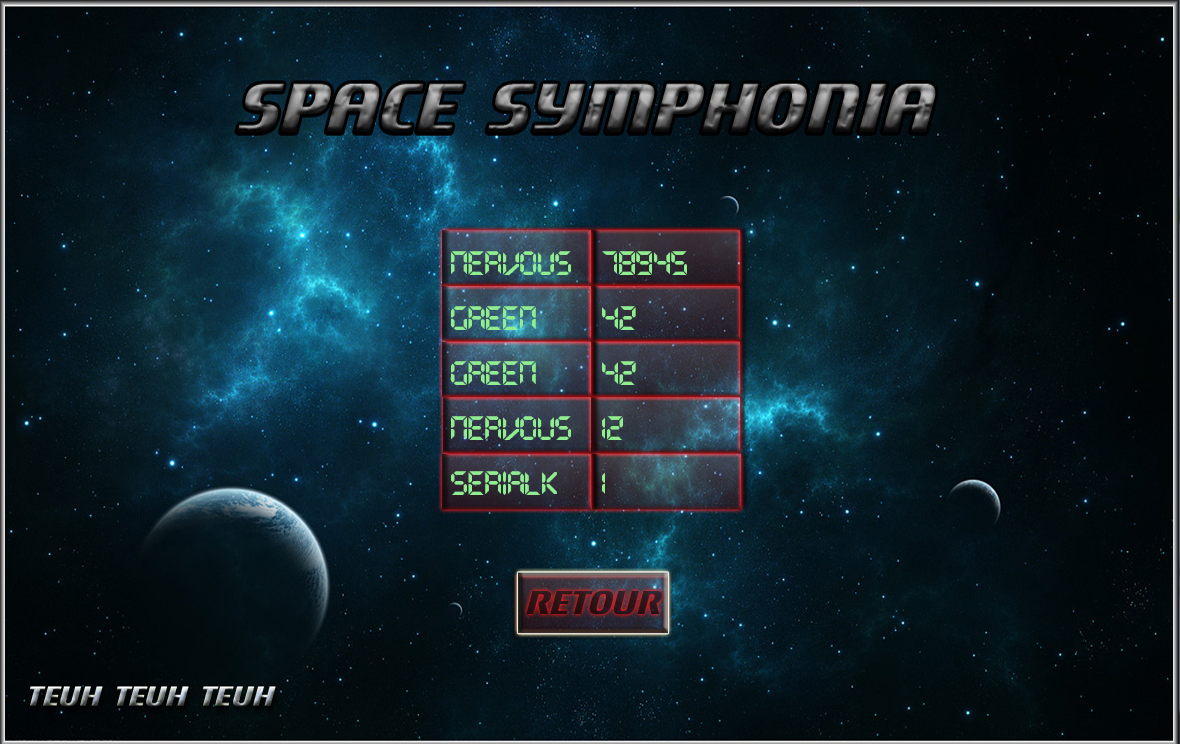
\includegraphics{images/score1.png}